\subsection{Enfoque general de la investigación}

La presente investigación adopta un enfoque metodológico de tipo \textbf{aplicado} con orientación \textbf{cuantitativa}, centrado en el diseño, la implementación y la evaluación de \textbf{ViaData — Medellín}: un instrumento virtual geoespacial para organizar, visualizar y proyectar la accidentalidad vial en Medellín a partir de datos históricos oficiales. El estudio articula de manera secuencial ingeniería de software, ciencia de datos y sistemas de información geográfica, de modo que los registros administrativos Mede se transformen en indicadores, mapas y escenarios orientativos con trazabilidad en los cálculos \cite{changotasig2023,lugo2025}.

A diferencia de un análisis puramente descriptivo, la metodología incorpora \textbf{analítica predictiva} con modelos estadísticos transparentes (OLS, estacional, Poisson, media móvil, bandas $\mu \pm 3\sigma$, ARIMA y SARIMA) y validación \textit{hold-out}, además de índices de priorización y carga territorial. Las proyecciones se interpretan como escenarios bajo estabilidad del patrón histórico filtrado: apoyan la planificación y la lectura comparativa, pero \textbf{no establecen causalidad} ni probabilidad individual de sufrir un siniestro \cite{oms2024,parraga2024}. La Figura~\ref{fig:diagrama-de-metodologia} resume las fases del proceso.

\begin{figure}[H]
	\centering
	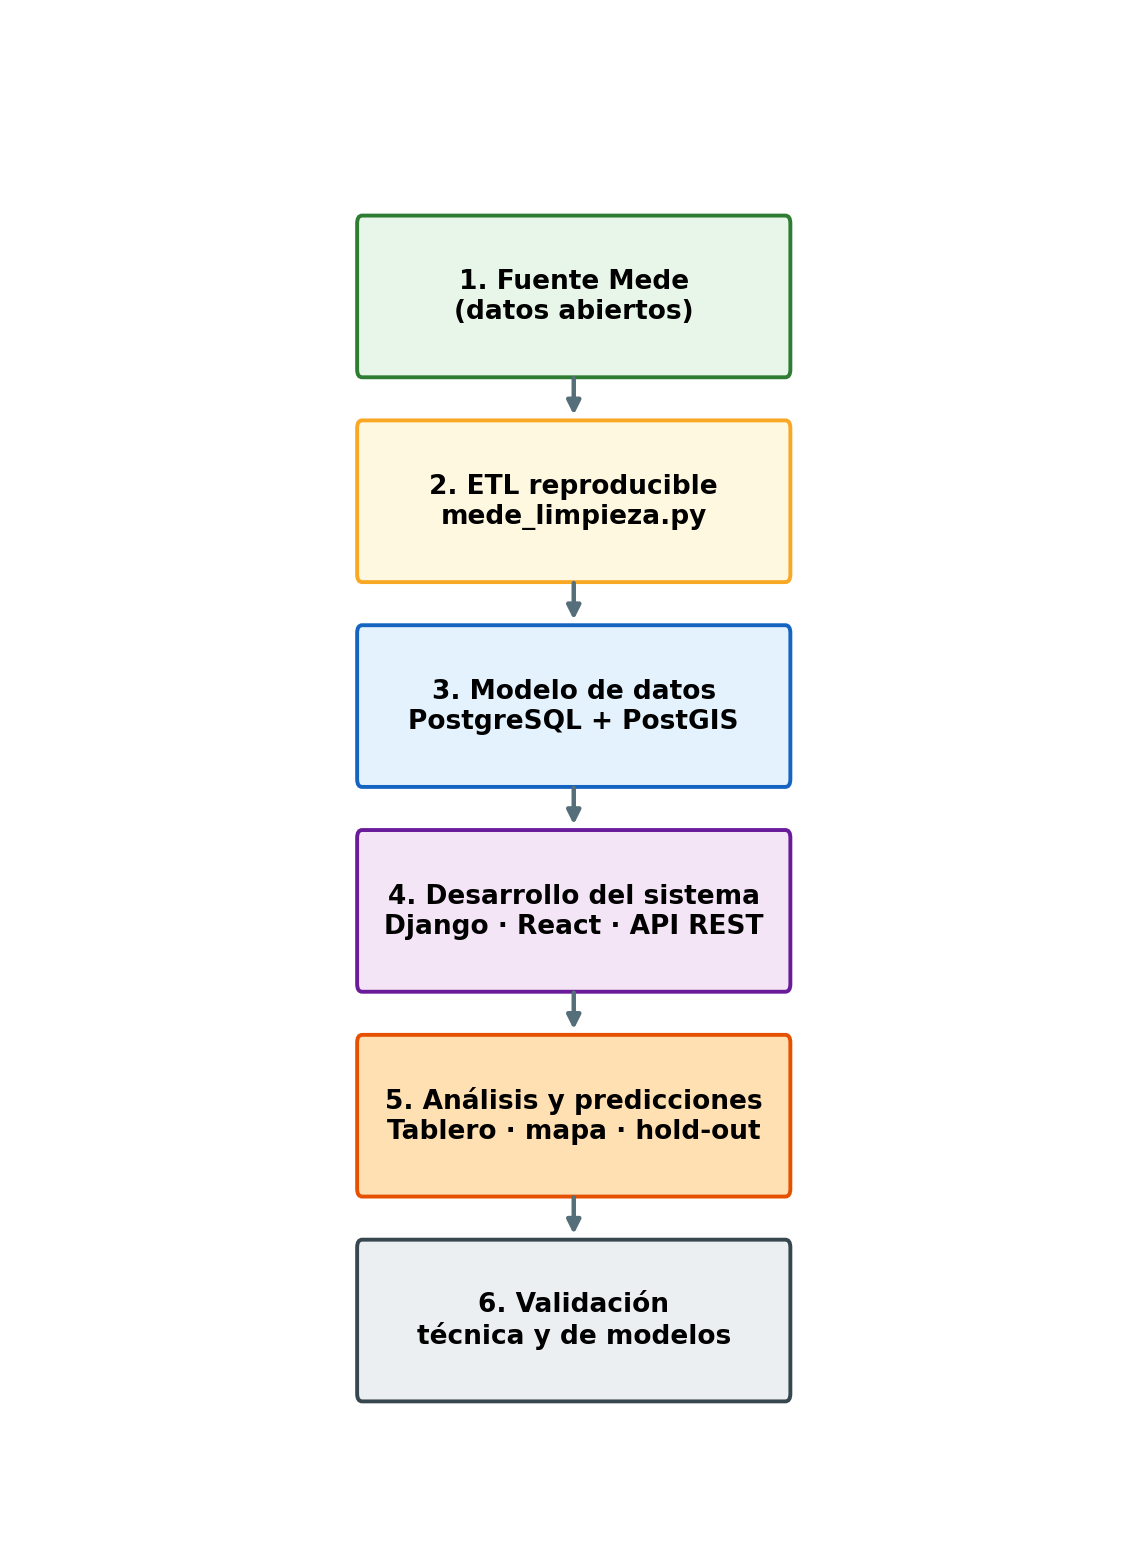
\includegraphics[width=0.62\linewidth]{images/fig_metodologia.png}
	\caption{Fases metodológicas de ViaData — Medellín}
	\label{fig:diagrama-de-metodologia}
\end{figure}

\subsection{Fuentes de datos y proceso ETL}

La fuente principal corresponde al conjunto de datos abiertos \textbf{Mede} publicado en la plataforma institucional de Medellín (\texttt{Mede\_Victimas\_inci.xlsx}), que concentra registros de incidentes y víctimas con variables temporales, territoriales, de gravedad y georreferenciación. El periodo típico cargado en la base del proyecto abarca aproximadamente \textbf{2014-01-01 — 2021-09-30}, con del orden de \textbf{160\,000+} incidentes con coordenadas válidas tras depuración, según el Excel y los indicadores de calidad del pipeline \cite{atancuri2024}.

La ingestión sigue un flujo \textbf{ETL reproducible} documentado y versionado. En primer lugar, el módulo \texttt{mede\_limpieza.py} concentra las reglas únicas de depuración (\texttt{depurar\_mede}), evitando duplicar lógica en otros scripts. A partir del Excel se genera \texttt{Mede\_Victimas\_inci\_depurado.csv}; el script \texttt{carga\_mede\_pgadmin.sql} realiza la carga idempotente a PostgreSQL; y los scripts PostGIS (\texttt{001}–\texttt{006}) más la carga de polígonos oficiales habilitan la asignación territorial espacial. Scripts auxiliares (\texttt{mede\_eda\_export.py}, \texttt{mede\_pipeline\_guiado.py}) apoyan el análisis exploratorio y la verificación de checkpoints. Este diseño garantiza que la memoria de grado, el EDA y la aplicación web describan el \textbf{mismo comportamiento} de limpieza \cite{provost2022}.

\begin{figure}[H]
	\centering
	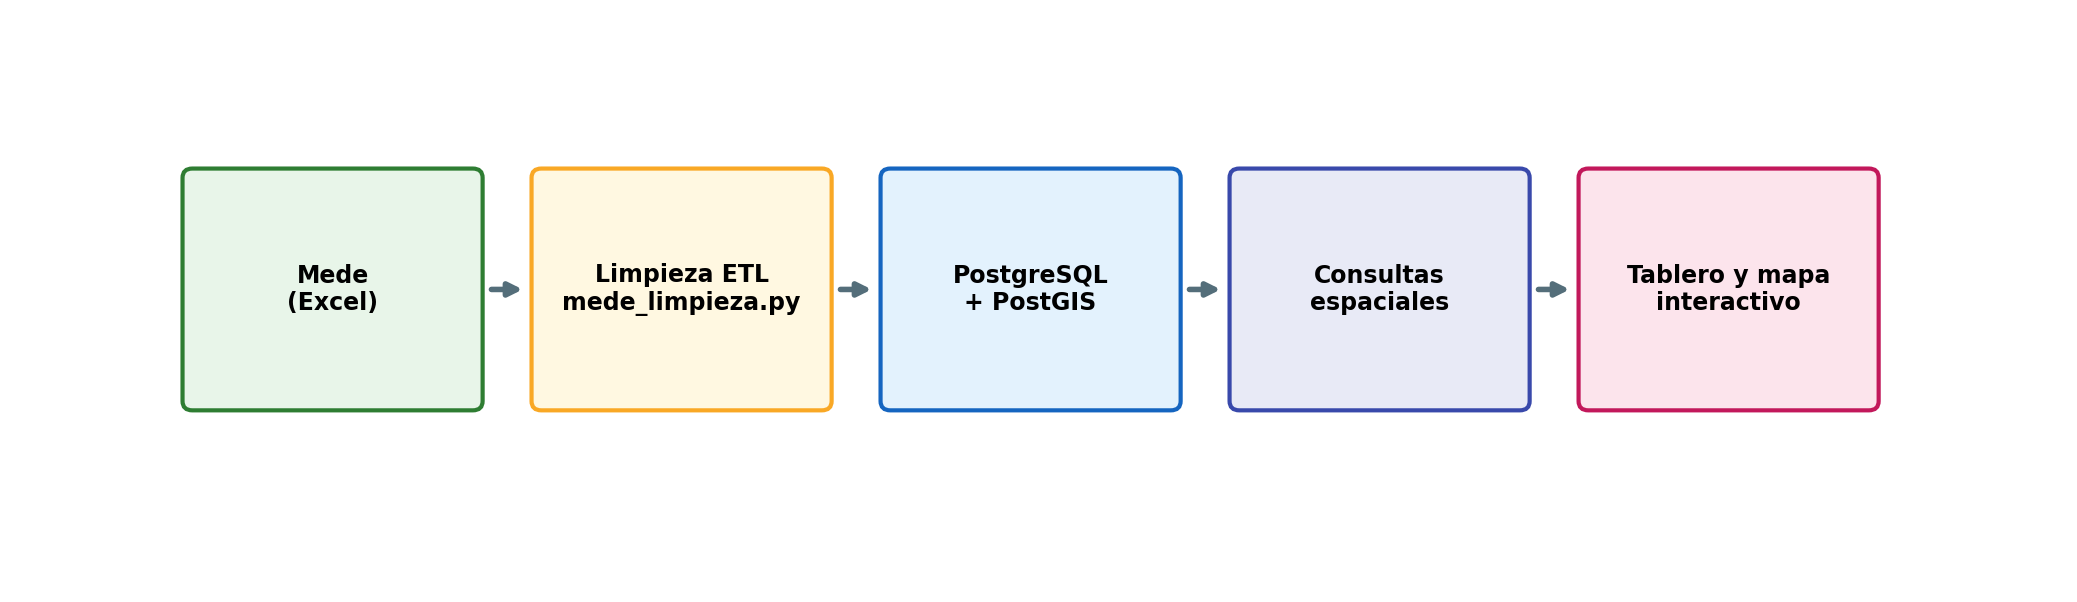
\includegraphics[width=0.95\linewidth]{images/fig_flujo_datos_geoespacial.png}
	\caption{Flujo de datos desde Mede hasta la visualización geoespacial}
	\label{fig:metodologia-flujo-etl}
\end{figure}

En la etapa de depuración se abordan inconsistencias de formato, valores faltantes, normalización de catálogos (tipo de incidente, clase, gravedad) y validación de coordenadas. La calidad del análisis posterior depende directamente de esta fase; el indicador G03 del sistema permite contrastar, una vez cargados los polígonos, la coincidencia entre el territorio declarado en el registro y el asignado espacialmente.

\subsection{Diseño del modelo de datos y territorio espacial}

El modelo relacional estructura la información en entidades normalizadas ---incidentes, víctimas y catálogos asociados--- con geometrías gestionadas por PostGIS. Cada incidente conserva atributos descriptivos y un punto geográfico cuando las coordenadas son válidas. ViaData — Medellín distingue dos modos de lectura territorial: \textbf{modo registro} (filtro por comuna o barrio declarado en Mede) y \textbf{modo espacial} (asignación por polígono oficial a partir de coordenadas), lo que permite evaluar la calidad cartográfica del dato y sostener agregaciones comparables en tablero, mapa y predicciones.

\subsection{Arquitectura e implementación del sistema}

El desarrollo adopta una \textbf{arquitectura monolítica} en Django que concentra autenticación JWT, API REST (Django REST Framework), lógica analítica y acceso a datos, mientras el frontend React (Vite) opera como aplicación de página única. Las apps \texttt{accounts}, \texttt{dashboard}, \texttt{agent} y \texttt{reports} cubren, respectivamente, usuarios y roles, KPIs y predicciones, asistente conversacional con herramientas sobre la API, y payloads para reportes imprimibles. GeoDjango y PostgreSQL/PostGIS soportan consultas espaciales; Leaflet y \texttt{react-leaflet} materializan capas en el cliente. Los cálculos predictivos emplean NumPy en rutinas propias y \textbf{statsmodels} para ARIMA/SARIMA; el ETL offline usa pandas según \texttt{requirements-etl.txt}. La Figura~\ref{fig:arquitectura-monolitica} del marco conceptual detalla el patrón MTV del backend.

\subsection{Procesamiento analítico y módulo de predicciones}

El procesamiento combina consultas SQL parametrizadas en tiempo de petición con rutinas numéricas en el backend. En el plano \textbf{descriptivo y diagnóstico}, el tablero y el mapa calculan KPIs, series mensuales, distribuciones por día y hora, densidades territoriales (G01--G02), rankings por comuna o barrio y concentraciones espaciales (G06/P14) mediante KDE o cuadrículas cuando el volumen lo permite \cite{xu2022,monar2025}.

El módulo de \textbf{predicciones} organiza cinco bloques analíticos con filtros compartidos (fechas, territorio, clase de incidente, exclusión opcional de mar–ago 2020):

\begin{itemize}
	\item \textbf{§1 Proyección mensual} (P01--P04): compara siete familias de modelos sobre conteos mensuales de incidentes, víctimas o fatales.
	\item \textbf{§2 Prioridad territorial} (P05): índice multicriterio fijo sobre el periodo filtrado, sin entrenamiento predictivo.
	\item \textbf{§3 Carga territorial} (P08--P10): proyección de volumen futuro por comuna o barrio.
	\item \textbf{§4 Proporción de fatales} (P07): modelos sobre el porcentaje de víctimas fatales.
	\item \textbf{§5 Patrones temporales} (P12--P13): reparto día$\times$hora a partir del total proyectado en §1.
\end{itemize}

La cadena de dependencias entre bloques se presenta en la Figura~\ref{fig:cadena-predictiva} del marco conceptual. El alcance deliberadamente \textbf{no incluye} ranking automatizado por vía o punto crítico ---ausente en Mede--- ni modelos de aprendizaje automático espacial avanzado; la ingesta de datos nuevos permanece como proceso manual reproducible.

\subsection{Protocolo de evaluación de modelos}

La evaluación predictiva distingue ajuste \textbf{in-sample} y validación \textbf{hold-out}: se reservan los últimos $N$ meses del rango, se entrena sin ellos y se mide el error al predecirlos. El hold-out es el \textbf{criterio principal} para seleccionar modelo en §1 y §4; se adopta como umbral exploratorio un MAPE hold-out $\leq 20\,\%$ (precisión estimada $\approx 100\,\% - \mathrm{MAPE}$), sin exigir R$^2 \geq 0{,}80$ en series mensuales perturbadas por la pandemia. La Figura~\ref{fig:holdout-validacion} del marco conceptual ilustra este esquema.

La Tabla~\ref{tab:config-evaluacion} resume la configuración estándar del escenario de referencia A; la Tabla~\ref{tab:protocolo-bloques} especifica la métrica y la decisión adoptada por bloque. Los scripts \texttt{llenar\_evaluacion\_seccion*.py} y los CSV en \texttt{evaluaciones/} aseguran reproducibilidad numérica; los resultados detallados se reportan en la sección de resultados.

\begin{table}[h]
	\centering
	\caption{Configuración estándar de evaluación predictiva (escenario A)}
	\label{tab:config-evaluacion}
	\small
	\begin{tabularx}{\linewidth}{@{}l X@{}}
		\toprule
		\textbf{Parámetro} & \textbf{Valor} \\
		\midrule
		Periodo de referencia & 2018-01-01 — 2021-09-30 \\
		Excluir mar–ago 2020 del ajuste & Sí (opción por defecto en la interfaz) \\
		Hold-out & 3 meses (6 opcionales en §1 y §4) \\
		Horizonte de proyección & 3 meses \\
		Escenarios §1 & A–I (ciudad, variable, territorio, clase, COVID, rangos cortos) \\
		\bottomrule
	\end{tabularx}
\end{table}

\begin{table}[h]
	\centering
	\caption{Protocolo de evaluación por bloque del módulo de predicciones}
	\label{tab:protocolo-bloques}
	\small
	\begin{tabularx}{\linewidth}{@{}l c X l@{}}
		\toprule
		\textbf{Bloque} & \textbf{¿Modelos?} & \textbf{Métrica principal} & \textbf{Decisión} \\
		\midrule
		§1 Proyección mensual & Sí (7 $\times$ 9 escenarios) & MAPE hold-out & SARIMA ciudad incidentes \\
		§2 Prioridad territorial & No (índice fijo) & Spearman índice$\leftrightarrow$frecuencia & P05 comunas referencia \\
		§3 Carga territorial & Sí (6 en A; estacional en B–G) & Spearman carga$\leftrightarrow$volumen & Estacional territorial \\
		§4 Proporción fatales & Sí (8 en A) & MAPE hold-out sobre \% & Estacional sobre \% \\
		§5 Patrones temporales & Hereda §1 & Spearman patrón obs.$\leftrightarrow$proy. & Patrón estable; hereda §1 \\
		\bottomrule
	\end{tabularx}
\end{table}

Para la proyección mensual de incidentes a nivel ciudad, el modelo adoptado tras la evaluación es \textbf{SARIMA$(2,1,3)(1,1,1)_{12}$} implementado con statsmodels, con media móvil de tres meses como alternativa interpretable. El índice P05 se valida por correlación de Spearman con la frecuencia observada en comunas de referencia; la carga territorial y los patrones día$\times$hora se evalúan por coherencia de ranking y estabilidad del patrón, respectivamente.

\subsection{Validación técnica del software}

Complementariamente a la evaluación de modelos, la metodología contempla \textbf{validación técnica del sistema}: pruebas automatizadas con \texttt{pytest} y \texttt{pytest-django} sobre las apps \texttt{dashboard}, \texttt{agent}, \texttt{accounts} y \texttt{reports}; verificación de endpoints críticos de la API; y revisión de desempeño en consultas frecuentes a PostgreSQL/PostGIS. Esta fase responde al objetivo específico de validar desempeño, seguridad y escalabilidad de la plataforma, y se complementa con la coherencia de indicadores y la utilidad de tablero, mapa y reportes para el análisis de accidentalidad.

En conjunto, el proceso metodológico integra desarrollo tecnológico, calidad del dato, analítica descriptiva/diagnóstica/predictiva y validación reproducible, transformando datos abiertos Mede en un instrumento geoespacial consultable que responde a los objetivos planteados y deja trazabilidad para extensiones futuras documentadas en trabajo futuro.

\subsection{Instrumentos y técnicas de recolección y análisis de datos}

La investigación se fundamenta en \textbf{fuentes secundarias} estructuradas: el dataset Mede como instrumento principal de recolección indirecta. No se aplican encuestas ni instrumentos de campo; la evidencia empírica proviene de registros administrativos ya consolidados por la institución.

Para el procesamiento se emplean Python (\texttt{pandas}, \texttt{numpy}) en el ETL offline; SQL y GeoDjango/PostGIS en consultas y agregaciones; NumPy y statsmodels en modelos de series; y bibliotecas de visualización en el cliente (Recharts, Leaflet). Las técnicas de análisis abarcan analítica descriptiva y diagnóstica (KPIs, distribuciones, índice P05), análisis geoespacial (densidad, coroplética, asignación territorial), modelado de conteos y series temporales con validación hold-out, y generación de reportes exportables. La reproducibilidad del ETL y de las evaluaciones numéricas constituye un criterio transversal del diseño metodológico.

\subsection{Población y muestra}

La \textbf{población} objeto de estudio está conformada por el conjunto total de registros de accidentes de tránsito ocurridos en Medellín y reportados en Mede dentro del periodo disponible en el dataset cargado. Incluye distintos tipos de incidente, actores viales, condiciones y niveles de gravedad según la estructura del archivo fuente.

Dado que el estudio se basa en datos secundarios, no se realiza muestreo probabilístico en sentido tradicional: se trabaja con la \textbf{totalidad de los registros} disponibles tras depuración (enfoque censal), lo que reduce sesgos de selección y permite analizar el fenómeno de manera integral \cite{oviedo2025}. Para fines analíticos, la plataforma aplica filtros temporales, geográficos y categóricos que segmentan la población en subconjuntos ---periodos, comunas, clases de incidente, rangos con o sin exclusión COVID--- sin constituir muestras independientes, sino estrategias de exploración y evaluación bajo escenarios documentados.
